\label{model}
In this section an example of a typical mathematical model for offline optimization will be presented along with a model, which allows for more dynamic systems.

The following, simplied, notation is used:

\begin{table}[!ht]
\begin{center}
\begin{tabular}{ll}
\hline
C & Common cycle time \\
$\theta_n$ & Offset of intersection $n$ \\
$\Psi$ & A set of signal settings \\
$\phi_{n,p}$ & Phase $p$ green time duration for intersection $n$  \\
$P_n$ & The number of phases at intersection $n$
\\ \hline
\end{tabular}
\end{center}
\caption{Notation}
\end{table}

The problem is now formulated as the minimization of a selected performance index (PI) in terms of a set of signal settings, $\Psi$, and a network of user equilibrium link flows, $\textbf{q*}(\Psi)$, which is dependent on the signal settings.

Teklu \cite{2} presents a model which is typical for offline optimizers:

\begin{eqnarray}
\min PI \left(  \Psi, \textbf{q*}\left( \Psi\right)  \right)
\end{eqnarray}
\begin{eqnarray}
\label{eqn:cycletimeconstraints} subject\;to:\;C_{min} \leq C \leq C_{max} \\
\label{eqn:offset} 0 \leq \theta_n \leq C-1\\
\label{eqn:greentimelimits} \phi_{n,p,min} \leq \phi_{n,r} \leq \phi_{n,p,max}\\
\label{eqn:commoncycledef} C = \sum_{p=1}^{P_n} \phi_{n,p}
\end{eqnarray}

In the article the chosen performance index is the travel time defined as the sum of flow multiplied by travel time on each link and $\Psi = \lbrace C,\theta,\phi \rbrace$. The interphase lost times are omitted for clarity reasons.

The sum of green time for all phases for an intersection must equal the common cycle time as seen in equation \ref{eqn:commoncycledef}. Equations \ref{eqn:cycletimeconstraints} and \ref{eqn:greentimelimits} are safeguards entered by traffic engineers to avoid extreme plans. Equation \ref{eqn:offset} relates the offset to the cycle time. Offset cannot exceed the common cycle time.

It is clear that this model does not consider phase sequences. Phases are simply enumerated and allocated green time - the order is assumed given. Furthermore the restrictive periodicity of the model can be seen clearly since $\phi$ cannot change as a function of time although, at least the order could actually be changed behind the scenes.

In a general, discrete time, model time steps are denoted by $t$. The network consists of $N \geq 1$ signal controlled intersections indexed by $n$.

In the model each signal is designated a phase for each time unit. Thus the concept of a cycle becomes virtual as they are no longer mandatory for calculating eg. the length of phases given the green splits.

Without a common cycle time - or individual cycle time, even - the offset parameter also disappears. However they can be made to exist virtually, in terms of a virtual cycle, and can thus be manipulated to excert the same behaviour. 
The main problem is during initialization when the system has just started. In this case it is possible synchronize intersections by delaying startup for those that would otherwise have a positive offset and vice versa for negative offset intersections. The same strategy can be used when increasing or decreasing the (virtual) cycle time for the arterial.

Phase sequences and green splits are unified by the specification of the phase in a timeslot, $t$, referred to as $p_n(t)$. For each intersection there will be a fixed number of phases, $P_n$, which are free from right-of-way conflicts. For a simple cross intersection with left-side driven vehicles (see figure \ref{fig:simple_intersection}) this number is 2: straight, left, and right turning flows in north and south directions for phase 1 and in east and west directions for phase 2.

\begin{figure}[!h]
\begin{center}
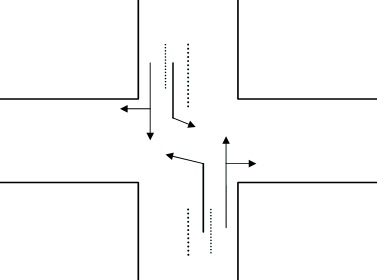
\includegraphics[scale=0.4]{simple_intersection.png} 
\end{center}
\label{fig:simple_intersection}
\caption{Simple intersection}
\end{figure}

Thus a specific phase $p = p_n(t) \in \lbrace 1,...,P_n \rbrace$ is selected for each timeslot. With this definition the green splits are implicit in the phase sequence. 

Now $\Psi = \lbrace \textbf{p} \rbrace $ and we can perform an optimization.

Satisfaction of minimum and maximum green times is the most common constraint, usually defined within a cycle. In this model the following equation must be satisfied:

$$
\forall p,n: \; T = \lbrace t: p_n(t) = p \rbrace \; st. \; cons(T) \wedge T_{min,p,n} \leq |T| \leq T_{max,p,n} 
$$
Thus $T$ is a set of points in time and the $cons$ function is defined by:
$$
cons(T) = 
\begin{cases}
true & if \;  \displaystyle\sum_{t \in T}{t} = � \cdot (\max T + \min T) \cdot (\max T - \min T + 1) \\
false & otherwise
\end{cases}
$$

That is, there must be a consecutive series of time slots (tested by using the Gaussian rule for summation of consecutive integers) in which phase $p$ is run.